\documentclass{article}

\usepackage{hyperref}
\usepackage{geometry}
\usepackage{changepage}
\usepackage{graphicx}
\usepackage[export]{adjustbox}
\usepackage{titlesec}
\usepackage{xcolor}
\hypersetup{
    colorlinks,
    linkcolor={red!50!black},
    citecolor={blue!50!black},
    urlcolor={blue!80!black}
}

\setlength\parindent{0pt} % noindet
\setcounter{secnumdepth}{4}

\geometry{legalpaper, margin=2cm}

\graphicspath{{../img/}}

\titleformat{\paragraph}
{\normalfont\normalsize\bfseries}{\theparagraph}{1em}{}
\titlespacing*{\paragraph}
{0pt}{3.25ex plus 1ex minus .2ex}{1.5ex plus .2ex}

\begin{document}

\large{\textbf{Dr Thomas Huet}}\\
%\begin{itemize}
\normalsize
EAMENA Researcher and Database Manager\\
\small
$\cdot$Endangered Archaeology in the Middle East and North Africa\\
\normalsize
University of Oxford, School of Archaeology\\
\small
$\cdot$2 South Parks Road, Oxford OX1 3TG, United Kingdom
\normalsize
%\end{itemize}
\\
\smash{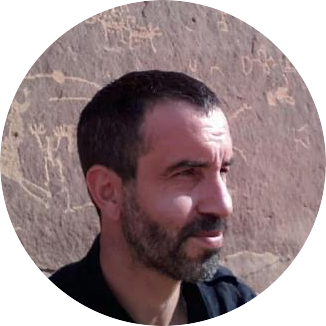
\includegraphics[width=3.5cm, right]{id-r}}

\includegraphics[scale=0.025]{gmail} \quad \href{mailto:thomas.huet@arch.ox.ac.uk}{thomas.huet@arch.ox.ac.uk} \& \href{mailto:thomashuet7@gmail.com}{thomashuet7@gmail.com}\\

\includegraphics[scale=0.01]{webpro} \quad \href{https://archit.web.ox.ac.uk/people/dr-thomas-huet}{School of Archaeology} \& \href{https://eamena.org/people/dr-thomas-huet}{EAMENA project}\\

\includegraphics[scale=0.007]{orcid} \quad \href{https://orcid.org/0000-0002-1112-6122}{0000-0002-1112-6122} \\

\includegraphics[scale=0.007]{github} \quad \href{https://github.com/zoometh/thomashuet.github.io/blob/main/README.md}{zoometh} \\

\includegraphics[scale=0.025]{gscholar} \quad \href{https://scholar.google.fr/citations?user=2hKEVaIAAAAJ}{2hKEVaIAAAAJ} \\

\includegraphics[scale=0.05]{rgate} \quad \href{https://www.researchgate.net/profile/Thomas\_Huet2}{Thomas\_Huet2} \\

\includegraphics[scale=0.005]{phone} \quad  \+ 44 (0)7 518 152 642 \\

\\

\begin{adjustwidth}{50pt}{50pt}
\begin{center}
\large{\textbf{Curriculum Vitae}}\\
\large{Prehistory, Cultural Heritage \& Computational Archaeology} 
\end{center}
\end{adjustwidth}

\section{ACADEMIC \textit{\&} PROFESSIONAL POSITIONS (since 2013-)}

\textbf{2021-23 }EAMENA Researcher and Database Manager, University of Oxford, School of Archaeology, 2 South Parks Road, Oxford OX1 3TG, United Kingdom, 1 November-...
\smallbreak
\textbf{2021 }Research Support (Technician T\`{e}cnic Especialista de Suport a la Recerca - TEC), Departament de Prehist\`oria, Universitat Aut\`{o}noma de Barcelona (UAB), Spain, 1 July-31 October.
\smallbreak
\textbf{2020 }Co-responsible of the survey of the medieval engravings of Sauri (Catalonia, Spain), 2${}^{nd\ }$campaign, Universitat Aut\`{o}noma de Barcelona (UAB), Spain, 19-24 October.
\smallbreak
\textbf{2019-20 }Researcher at Archa\"{i}os company, in charge of the database integration for the survey of Al-'Ula, Saudi-Arabia (Archa\"{i}os, AFALULA, RCU), 1 June - 1 June
\smallbreak
\textbf{2019 }Co-responsible of the survey of the medieval engravings of Sauri (Catalonia, Spain), 1${}^{st\ }$campaign, Universitat Aut\'{o}noma de Barcelona (UAB), Spain, 15 September-15 October.\\
\textbf{--- }Study Engineer (IE), UMR 8546 CNRS/PSL-AOrOc, Paris and Allones, 1 June - 1 July.
\smallbreak
\textbf{2018 }Research Engineer (IR), UMR 7264 CEPAM-CNRS, Universit\'{e} Nice Sophia-Antipolis, project \textit{C\'{e}ramiques Imprim\'{e}es de M\'{e}diterran\'{e}e occidentale} (CIMO), 1 May-30 August and 1 October-30 November. \\
\textbf{--- }Research Engineer (IR), UMR 5140 ASM-CNRS, Universit\'{e} Paul Val\'{e}ry Montpellier 3, project \textit{EpiSpat} (aka \textit{ArchaEpigraph}), LabEx ARCHIMEDE, 1 April-1 May, and 1-30 September.
\smallbreak
\textbf{2017-18 }Research stay. Recording techniques of rock-art and engraved steles of South-West Iberic peninsula (\textit{Tecniques d'enregistrament de l'art rupestre de les esteles gravades del Sud-oest de la Peninsula ibèrica}), Archaeology of Social Dynamics (ASD), Instituci\'{o}n Mil\`{a} y Fontanals (IMF) - Consejo Superior de Investigaciones Cient\'{i}ficas (CSIC), Barcelone, 1 September-30 May.
\smallbreak
\textbf{2015 }Auditor in the research seminar "Regards crois\'{e}s sur la notion de paysage", lector: S. Robert, EHESS, March-June.\textbf{}
\smallbreak
\textbf{2014 }Research Engineer (IR), project \textit{Archaepigraph} project, UMR 6249 Chrono-Environnement, Universit\'{e} de Franche-Comt\'{e}, dir. M.-J. Ouriachi and L. Nuninger, 1 September-30 October.
\smallbreak
\textbf{2013-14 }Study Engineer (IE), USR CNRS - UB 3516, GeoBFC platform, MSH de Dijon, Universit\'{e} de Bourgogne, project OH-FET (Historical Object, Function, Space, Time), dir. L. Saligny, 1 June-31 May.

\section{EDUCATION}

\textbf{2006-12 }PhD History and Archaeology, title: 'Organisation spatiale et s\'{e}riation des gravures piquet\'{e}es du mont Bego', first level of distinction (mention tr\'{e}s honorable avec les f\'{e}licitations du jury), 29 May 2012, Universit\'{e} Nice Sophia-Antipolis, UMR 7264 CEPAM-CNRS, HALtheses: \href{https://tel.archives-ouvertes.fr/tel-00712290}{tel-00712290}.
\smallbreak
\textbf{2005-6 }Master 2 Research History and Archaeology, title: '\'{E}tude des gravures protohistoriques de la zone des lacs (zones I, II, III et V) de la r\'{e}gion du mont Bego, Tende, Alpes-Maritimes', mention bien. Universit\'{e} Nice Sophia-Antipolis, UMR 7264 CEPAM-CNRS, HALtheses: \href{https://tel.archives-ouvertes.fr/tel-00715386}{tel-00715386}.
\smallbreak
\textbf{2004-5 }DUT G'{e}nie informatique (University Diploma of Technology, Informatics Engineering), Conservatoire National des Arts et M\'{e}tiers (CNAM), Paris.
\smallbreak
\textbf{2003 } Topography diploma, Universitad de Ingenier\'{i}a, Lima, Peru.
\smallbreak
\textbf{2002 } Maîtrise Archaeology (Master 1 Archaeology), Université Paris IV, Paris-Sorbonne, Paris.
\smallbreak
\textbf{2001 } Licence Archaeology, Université Paris IV, Paris-Sorbonne, Paris.
\smallbreak
\textbf{2000 } DEUG Archaeology and History of Art, Université Paris IV, Paris-Sorbonne, Paris.

\section{PRIZES AND AWARDS}

\textbf{2023 }Meyerstein Fund.
\smallbreak
\textbf{2013 }PhD prize for publication. CASDEN -- Banque Populaire (UFR LSH, Universit\'{e} Nice Sophia-Antipolis).
\smallbreak

\section{PUBLICATIONS}

\begin{center}------------ Journals articles ------------\end{center}
$\bullet$ Pasqualini A., \textbf{Huet T.} and M.-J. Ouriachi (\textit{\textbf{submitted}}). Une base de données informatique dédiée au programme Epispat, \textit{in} Ouriachi M.-J. et Pellecuer C. (eds), \textit{Actes de la Table-ronde de cl\^{o}ture du programme Epispat, 21-22 nov. 2019, Hi\'{e}rarchie sociale et d\'{e}veloppement territorial en Gaule Narbonnaise et dans les provinces voisines : enqu\^{e}tes au croisement de l'\'{e}pigraphie et de l'arch\'{e}ologie spatiale}, Revue Arch\'{e}ologique de Narbonnaise.
\smallbreak
$\bullet$ Gassiot Ballbè E., Augé Martínez O., Lapedra Grau S., \textbf{Huet T.}, Sánchez Bonastre X. and R. Martí Castelló (\textit{\textbf{submitted}}). Paisatges de conflicte i poder. Els gravats medievals del Solà de Saurí, (Pallars Sobirà), \textit{Tribuna d'Arqueologia}
\smallbreak
$\bullet$ Charbonnier J., Kanhoush Y., Gravier J., Gourret G., Achouche I., Bernollin V., Boudia S., Bucci W., Chiti B., Clauss-Balty P., Colard V., Devaux E., Dupont-Delaleuf A., De Smet A., Furstos C., Goy J., Haze M., Hofstetter T., Housse R., \textbf{Huet T.}, Marquaire C., Paola Pellegrino M., Raad C., Ricart J.-D., Rosak A., Saïd A.F., Serres D., Siméon P., Tourtet F. and J. Giraud (\textit{\textbf{submitted}}). Mapping an Arabian oasis: first results of UCOP systematic survey of al-'Ūla Valley
(2019-2021), \textit{Proceedings of the Seminar for Arabian Studies (PSAS)}
\smallbreak
$\bullet$ Cicolani V., \textbf{Huet T.} and L. Zamboni (\textit{\textbf{submitted}}). Centre et marges, une approche critique : modélisation des interactions entre entités culturelles en Italie du Nord à l'âge du Fer, \textit{Comit\'{e} des Travaux Historiques et Scientifiques \'{e}ditions} (CTHS)
\smallbreak
$\bullet$ \textbf{Huet T.}, Cubas M., Gibaja J.F., Oms F.X. and N. Mazzucco (\textbf{2022}). NeoNet Dataset. Radiocarbon Dates for the Late Mesolithic/Early Neolithic Transition in the North Central-Western Mediterranean Basin, \textit{Journal of Open Archaeology Data}, DOI: \href{http://doi.org/10.5334/joad.87}{10.5334/joad.87}.
\smallbreak
$\bullet$ \textbf{Huet T.}, Pozo J. M. and Alexander C. (\textbf{2021}), Analysis of Prehistoric Iconography with the R package \textit{iconr}, \textit{Journal of Open Statistical Software}, \href{https://joss.theoj.org/papers/10.21105/joss.03191}{10.21105/joss.03191}.
\smallbreak
$\bullet$ Nieto-Espinet A., \textbf{Huet T.}, Trentacoste A., Guimaraes S., Orengo H. and S. Valenzuela-Lamas (\textbf{2021}). Resilience and livestock adaptations to demographic growth and technological change: A diachronic perspective from the Late Bronze Age to Late Antiquity in NE Iberia, \textit{PlosONE}, DOI: \href{https://doi.org/10.1371/journal.pone.0246201}{10.1371/journal.pone.0246201}
\smallbreak
$\bullet$ Iba\~{n}ez J.J., Mu\~{n}iz J., \textbf{Huet T.}, Borrell Terra F.,.Santana Y., Teira Mayolini L.C. and R. Rosillo (\textbf{2020}). Flint Figurines in the Early Neolithic site of Kharaysin (Early 8th Millennium BC, Jordan), \textit{Antiquity Journal, 94, 376}, 880-899, DOI: \href{https://doi.org/10.15184/aqy.2020.78}{10.15184/aqy.2020.78}.
\smallbreak
$\bullet$ Cicolani V. and \textbf{T. Huet} (\textbf{2019}). Essai de mod\'{e}lisation des \'{e}changes et des r\'{e}seaux de circulation dans les Alpes centrales au premier \^{a}ge du Fer, \textit{in} Deschamps M., Costamagno S., Milcent P.-Y., Pétillon J.-M., Renard C. and N. Valdeyron (dir.) "La conqu\^{e}te de la montagne : des premi\'{e}res occupations humaines \`{a} l'anthropisation du milieu", \textit{Comit\'{e} des Travaux Historiques et Scientifiques \'{e}ditions} (CTHS), DOI: \href{https://books.openedition.org/cths/7827}{10.4000/books.cths.7827}.
\smallbreak
$\bullet$ \textbf{Huet T.} (\textbf{2018}). Geometric Graphs to Study Ceramic Decoration\textit{, in} M. Matsumoto and.E. Uleberg (eds), Exploring Oceans of Data, \textit{Proceedings of the 44${}^{nd\ }$Conference on Computer Applications and quantitative Methods in Archaeology} (CAA2016), Oxford : Archaeopress Archaeology, 311-323, HAL: \href{https://hal.archives-ouvertes.fr/hal-02913656}{hal-02913656}
\smallbreak
$\bullet$ \textbf{Huet T.} (\textbf{2016}). New perspectives on the chronology and the meaning of Mont Bego's rock-art (Alpes-Maritimes, France), \textit{Cambridge Archaeological Journal} 41, 1-23, DOI: \href{https://doi.org/10.1017/s0959774316000524}{10.1017/s0959774316000524}.
\smallbreak
$\bullet$ \textbf{Huet T.} and N. Bianchi (\textbf{2016}). Reticolati, pelli e mappe topografiche, lo stato della ricerca al monte Bego, \textit{Bollettino del Centro Camuno di Studi Preistorici} 41, 31-43, ISSN 1594-7084 \href{http://www.ccsp.it/web/infoccsp/bcsp/bcsp41_preview.pdf}{
\includegraphics[scale=0.02]{link_darkblue.png}}.
\smallbreak
$\bullet$ \textbf{Huet T.} and N. Bianchi (\textbf{2016}). A study of the Roche de l'Autel's pecked engravings, Les Merveilles sector, Mont Bego area (Alpes-Maritimes, France), \textit{Journal of Archaeological Sciences: Reports} 5, 105-118, DOI: \href{https://doi.org/10.1016/j.jasrep.2015.11.006}{10.1016/j.jasrep.2015.11.006}.
\smallbreak
$\bullet$ \textbf{Huet T.} (\textbf{2016}). S\'{e}riation des gravures piquet\'{e}es du mont Bego, \textit{Archeologia e Calcolatori} 27, 65-83, DOI: \href{https://doi.org/10.19282/AC.27.2016.02}{10.19282/AC.27.2016.02}.
\smallbreak
$\bullet$ \textbf{Huet T.} (\textbf{2015}). Le incisioni a martellina del monte Bego: approcci geografici e quantitativi, \textit{Archeologia Postmedievale} 17, 329-338, ISSN 1592-5935 \href{https://www.insegnadelgiglio.it/wp-content/uploads/2015/01/APM_17_libro-anteprima.pdf}{
\includegraphics[scale=0.02]{link_darkblue.png}}.
\smallbreak
$\bullet$ Saligny L., Granjon L., \textbf{Huet T.}, Simon G., Rodier X. and B. Lefebvre (\textbf{2015}). OH\_FET: A Computer Application for Analysing Urban Dynamics Over Long Time Spans, in Giligny F., Djindjian F., Costa L., Moscati P. and S. Robert (eds) \textit{Proceedings of the 42${}^{nd\ }$Conference on Computer Applications and quantitative Methods in Archaeology} (CAA2014), Oxford : Archaeopress Archaeology, 381-392, HAL: \href{https://hal.archives-ouvertes.fr/halshs-01146871}{halshs-01146871}.
\smallbreak
$\bullet$ \textbf{Huet T.} and C. Alexander (\textbf{2015}). M\'{e}thodes informatiques pour l'\'{e}tude des gravures rupestres~: les exemples du Valcamonica (Italie) et du mont Bego (France), in Cervel M., Rousseau L. and M. Nordez (eds) \textit{Recherches sur l'\^{a}ge du Bronze. Nouvelles approches et perspectives. Actes de la journ\'{e}e d'\'{e}tude de l'APRAB, Bulletin de l'APRAB, suppl. 1}, 15-29 
\href{https://www.researchgate.net/publication/347437308_Methodes_informatiques_pour_l'etude_des_gravures_rupestres_les_exemples_du_Valcamonica_Italie_et_du_mont_Bego_France}{
\includegraphics[scale=0.02]{link_darkblue.png}}.
\smallbreak
$\bullet$ Ouriachi M.-J., Favory F., Garmy P., Ouzoulias P., Pasqualini A., Christol M., \textbf{Huet T}., Nuninger L., Bertoncello F. and R. H\"{a}ussler (\textbf{2014}). ArchaEpigraph : l'\'{e}pigraphie spatiale au service de l'\'{e}tude des dynamiques des territoires, in \textit{Revue arch\'{e}ologique de Narbonnaise}, tome 47, pp. 35-49, DOI: \href{https://doi.org/10.3406/ran.2014.1897}{10.3406/ran.2014.1897}.
\smallbreak
$\bullet$ \textbf{Huet T.} (\textbf{2014}). Use of quantitative methods to study an Alpine rock art site: the Mont Bego region, in Earl G., Sly T., Chrysanthi A., Murrieta Flores P., Papadopoulos C., Romanowska I. and D. Wheatley (eds) \textit{Proceedings of the 40${}^{th}$ Conference on Computer Applications and quantitative Methods in Archaeology} (CAA2012), Southampton, UK, 26-30 March 2012, Amsterdam : Pallas Publications, 584-591.
\smallbreak
$\bullet$ \textbf{Huet T.} (\textbf{2014}). Organisation spatiale et s\'{e}riation des gravures piquet\'{e}es du mont Bego~-- R\'{e}sum\'{e} de th\'{e}se, \textit{Bulletin de la Soci\'{e}t\'{e} Pr\'{e}historique Fran\c{c}aise} 110, 146-148, \href{https://www.persee.fr/doc/bspf_0249-7638_2013_num_110_1_14242}{
\includegraphics[scale=0.02]{link_darkblue.png}}.

\begin{center}------------ Books ------------ \end{center}
\smallbreak
$\bullet$ \textbf{Huet T.} (\textbf{2017}). \textit{Les gravures piquet\'{e}es du mont Bego (Alpes-Maritimes). Organisation spatiale et s\'{e}riation (6e -- 2e mill\'{e}naire av. J.-C.)}, M\'{e}moire de la Soci\'{e}t\'{e} Pr\'{e}historique Fran\c{c}aise (SPF) 63, 166 p., ISBN : 2-913745-71-7 \href{http://www.prehistoire.org/shop_515-40342-0-0/m63-2017-les-gravures-piquetees-du-mont-bego-alpes-maritimes-organisation-spatiale-et-seriation-vie-iie-millenaire-av.-j.-c.-t.-huet.html}{
\includegraphics[scale=0.02]{link_darkblue.png}}

\bigbreak
\begin{center}------------ Book chapters ------------\end{center}
\smallbreak
$\bullet$ Binder D., Gomart L., \textbf{Huet T.}, Ka{\v{c}}ar S., Maggi R., Manen C., Radi G., and Tozzi C. with the collaboration of Mutoni I.M., Natali E. and C. Panelli (\textbf{2022}). Le complexe de la C\'{e}ramique imprim\'{e}e de M\'{e}diterran\'{e}e centrale et occidentale : une synthèse chrono-culturelle (7e et 6e millénaires BCE), in Binder D. and C. Manen (dir), \textit{C\'{e}ramiques imprim\'{e}es de M\'{e}diterran\'{e}e occidentale (6e mill\'{e}naire BCE) : Donn\'{e}es, approches et enjeux nouveaux. Actes des journ\'{e}es de la Soci\'{e}t\'{e} Pr\'{e}historique Fran\c{c}aise, Nice, 18-20 mars 2019}, Paris: Soci\'{e}t\'{e} Pr\'{e}historique Fran\c{c}aise, p. 27-104, ISSN: 2263-3847, SPF: \href{https://www.prehistoire.org/515_p_57657/accEs-libre-seance-18-ceramiques-imprimees-de-mediterranee-occidentale.html}{spf-515}
\smallbreak
$\bullet$ Lanaspa J. R., Conte I. C., Gassiot Ballbè E., Mazzucco N., \textbf{Huet T.}, Olomi A. and J. Borràs (\textbf{2022}). Artiga Viturián, un nuevo yacimiento del Neolítico Antiguo en Sobrarbe (Huesca) in IV Congreso CAPA, Arqueología Patrimonio Aragonés, 29–36, ISBN: 978-84-09-41553-3.
\smallbreak
$\bullet$ Alexander C., Maretta A., \textbf{Huet T.} and C. Chippindale (\textbf{2021}). Rules of ordering and grouping in the 'pitoti', the later prehistoric rock-engravings of Valcamonica (BS), Italy: from solitary figures through clusters, graphic groups, and scenes to narrative, in I. Davidson and A. Nowell (eds), \textit{Making scenes: global perspectives on scenes in rock art}, London: Berghahn Books, p. 259-276 \href{https://www.berghahnbooks.com/title/DavidsonMaking}{
\includegraphics[scale=0.02]{link_darkblue.png}}.
\smallbreak
$\bullet$ \textbf{Huet T.} (\textbf{2018}). Une revue de l'iconographie du d\'{e}but du N\'{e}olithique \`{a} la fin de l'\^{a}ge du Bronze (ca. 5700-750 av. J.-C.) en France, \textit{in} Guilaine J. et D. Garcia (dir.), \textit{La Protohistoire de la France}, ed. Hermann, Paris, p. 221-249, HAL: \href{https://hal.archives-ouvertes.fr/hal-01983284}{hal-01983284}.
\bigbreak

\subsection*{Scientific Conferences \textit{\&} Seminars (2014-)}
\begin{center}(\textbf{i}) \textbf{i}nternational audience {\textbar} (\textbf{n}) \textbf{n}ational audience \end{center}
\smallbreak
\begin{center}------------ Organisation ------------\end{center}
\textbf{2023 }GMPCA, Session n$\mathrm{{}^\circ}$ 3.1: \textit{Gestion de jeux de données}. A. Pasqualini, M. Lebon, \textbf{T. Huet}, XXIVe colloque du \textit{GMPCA : Archéométrie 2023}, Nice, France, 17-21 April (\textbf{i})
\smallbreak
\textbf{-- }CAA2023, Session n$\mathrm{{}^\circ}$ 12: \textit{Chronological modelling: formal methods and research software}. E. Levy, \textbf{T. Huet}, F. Thiery, A. W. Mee, International congress of the \textit{Computer Applications and Quantitative Methods in Archaeology}, Amsterdam, Netherlands, 3-6 April \href{https://historical-time.github.io/caa23/s12/pres/#/title-slide}{
\includegraphics[scale=0.02]{link_darkblue.png}} (\textbf{i}).
\smallbreak
\textbf{2022 }CAA2022, Session n$\mathrm{{}^\circ}$ 07: \textit{"Cultural Heritage data across borders. Web-based management platforms for immovable cultural heritage in the global south"}. \textbf{T. Huet}, C. El Safadi, B. Rouhani and A. Smith, International congress of the \textit{Computer Applications and Quantitative Methods in Archaeology}, University of Oxford, UK, 8-11 August \href{https://eamena-project.github.io/reveal.js/projects/caa22s07.html}{
\includegraphics[scale=0.02]{link_darkblue.png}} (\textbf{i}). 
\smallbreak
\textbf{--- }9${}^{th}$ Seminar of Technology Prehistoric:\textit{"Confocal microscopy for the analysis of wear on tools and teeth in Prehistory"}. F. Pichon, J.J. Ibáñez, H. Arashi, H. Xhauflair, F. Estebaranz-Sanchez, L. Martinez, N. Mazzucco, A. Zupancich, \textbf{T. Huet} and S. J. Manchon, 2-4 May, Institute Milá y Fontanals (CSIC), Barcelona, Spain (\textbf{i})
\smallbreak
\textbf{2016 }S\'{e}minaire d'\'{e}quipe ASM-CNRS (UMR 5140), \'{e}quipe Soci\'{e}t\'{e}s de la Pr\'{e}histoire et de la Protohistoire: \textit{Analyser et interpr\'{e}ter les d\'{e}cors des c\'{e}ramiques pr\'{e}- et protohistoriques. Approches crois\'{e}es}. \textbf{T. Huet}, T. Lachenal and K. Peche-Quichilini, Universit\'{e} Paul-Val\'{e}ry, Montpellier, 27 May (\textbf{n})
\smallbreak
\textbf{2014 }CAA2014, Session n$\mathrm{{}^\circ}$ 20: \textit{"(Re)building past networks: archaeological science, GIS and network analysis"}. \textbf{T. Huet}, C. Alexander, S. Robert and E. Mermet, 42${}^{nd}$ international congress of the \textit{Computer Applications and Quantitative Methods in Archaeology}, Universit\'{e} Sorbonne, France, 22-25 April (\textbf{i})
\bigbreak

\begin{center}------------ Communications (invited) ------------\end{center}
\smallbreak

\textbf{2022 }"Analysis of Prehistoric Iconography with the R package iconr". \textbf{T. Huet}, Digital Archaeology seminar, Durham University, Durham, 28 November \href{http://shinyserver.cfs.unipi.it:3838/durham/_site/#/title-slide}{
\includegraphics[scale=0.02]{link_darkblue.png}} (\textbf{n}).
\smallbreak
\textbf{--- }"Mont Bego. A protohistoric rock-art site in the Southern Alps". \textbf{T. Huet}, \textit{Dipartimento di Civilt\'{a} e forme del Sapere}, Universit\'{a} di Pisa, Pisa, 14 April (\textbf{n}).
\smallbreak
\textbf{2017 }"Les repr\'{e}sentations d'attelages \`{a} l'\^{a}ge du Bronze (Espagne, France, Italie), dans le cadre du \textit{S\'{e}minaire de formation doctorale du r\'{e}seau interdisciplinaire AniMed}, University seminar, Universit\'{e} Paul-Val\'{e}ry, 26 January (\textbf{n}).
\smallbreak
\textbf{2015 }"Data Paths". \textbf{T. Huet}, University workshop, Z\'{a}pado\v{c}esk\'{a} Univerzita (\textit{University of West Bohemia}), Pilsen, Czech Republic, 12 March (\textbf{i}).
\smallbreak


\begin{center}------------ Communications ------------\end{center}
\smallbreak
\textbf{2023 }"EAMENA, a massive and open data information system for endangered archaeology and cultural heritage". B. Finlayson, B. Rouhani, \textbf{T. Huet}, M. Fradley, S. Neogi, M. Holloway and A. Wilson, \textit{Session 3.1: Gestion de jeux de données} - International congress of the \textit{Groupe des Méthodes Pluridisciplinaires Contribuant à l'Archéologie} (GMPCA), Nice, France, 17-21 April \href{https://eamena-project.github.io/eamena-arches-dev/talks/2023-gmpca/pres/#/title-slide}{
\includegraphics[scale=0.02]{link_darkblue.png}} (\textbf{i}).
\smallbreak
\textbf{--- }"Le projet CENTAURO: Introduction des équidés, hybridation et intensification agricole dans la vallée de l'Èbre du Néolithique final à l'époque romaine". A. Nieto-Espinet, I. Aguilera Aragón, N. Alonso, A. Castellano, L. Font, I. Gil, A. Grandal D'anglade, \textbf{T. Huet}, ..., \textit{Session 2.2: Exploitation et gestion des ressources végétales et animales} - International congress of the \textit{Groupe des Méthodes Pluridisciplinaires Contribuant à l'Archéologie} (GMPCA), Nice, France, 17-21 April \href{https://gmpca2023.sciencesconf.org/}{
\includegraphics[scale=0.02]{link_grey.png}} (\textbf{i}).
\smallbreak
\textbf{--- }"Discussing the need for a new CAA Special Interest Group on chronological modelling". \textbf{T. Huet}, E. Levy, F. Thiery and A. Mees, \textit{S12. Chronological modelling: formal methods and research software} - International congress of the \textit{Computer Applications and Quantitative Methods in Archaeology} (CAA2023), Amsterdam, 3-6 April \href{https://historical-time.github.io/caa23/sig/pres}{
\includegraphics[scale=0.02]{link_darkblue.png}} (\textbf{i}).
\smallbreak
\textbf{--- }"From thesaurus to semantic network: make (re)usable the ANRJCJC Itineris data". V. Cicolani, \textbf{T. Huet}, G. Reich and S. Durost, \textit{S29. How do we ensure archaeological data are usable and Reusable, and for whom? Putting the R in FAIR for archaeology's data} - International congress of the \textit{Computer Applications and Quantitative Methods in Archaeology} (CAA2023), Amsterdam, 3-6 April \href{https://anr-itineris.github.io/itineris/talk/caa-2023/thesaurus/pres/#/title-slide}{
\includegraphics[scale=0.02]{link_darkblue.png}} (\textbf{i}).
\smallbreak
\textbf{--- }"Statistics and Computer Scripts in Archaeology". \textbf{T. Huet}, Graduate Skills Seminars (GAO), Institute of Archaeology, Oxford, 19 October \href{http://shinyserver.cfs.unipi.it:3838/teach/stats/gao/_site/#/title-slide}{
\includegraphics[scale=0.02]{link_darkblue.png}} (\textbf{n}).
\smallbreak
\textbf{--- }"A workflow for reproducible use-wear analysis with open-source software". \textbf{T. Huet}, J.J. Ibáñez, A. Zupancich and F. Estebaranz-Sánchez, International congress of the \textit{Computer Applications and Quantitative Methods in Archaeology}, School of Archaeology, University of Oxford, UK, 8-11 August \href{https://zoometh.github.io/reveal.js/projects/caa_3dlithic}{
\includegraphics[scale=0.02]{link_darkblue.png}} (\textbf{i}).
\smallbreak
\textbf{--- }"Analyzing the EAMENA database with R and Python scripted routine". \textbf{T. Huet}, K. Hopper and W. Deadman, \textit{EAMENA Workshop}, School of Archaeology, University of Oxford, UK, 7-8 July \href{https://eamena-project.github.io/reveal.js/projects/time.html}{
\includegraphics[scale=0.02]{link_darkblue.png}} (\textbf{n}).
\textbf{--- }"Centre et marges, une approche critique : modélisation des interactions entre entités culturelles en Italie du Nord à l'âge du Fer". V. Cicolani, \textbf{T. Huet} and L. Zamboni, 142${}^{e}$ congr\'{e}s du \textit{Comit\'{e} des Travaux Historiques et Scientifiques} (CTHS), Aubervilliers, 6 May (\textbf{n}).
\smallbreak
\textbf{2021 }"NeoNet. Database \& App". \textbf{T. Huet}, N. Mazzuco, M. Cubas, J.F. Gibaja and F.X. Oms, Origin, development and consolidation of the Neolithic in the Mediterranean region, EEHAR CSIC, Roma, 14-15 September \href{https://youtu.be/GM2niot0XwE?t=10700}{
\includegraphics[scale=0.2]{icon_youtube}} (\textbf{i}).
\smallbreak
\textbf{--- }"Human face depictions of Early Neolithic in the Near East". \textbf{T. Huet}, J.J. Ibáñez, J.M. Pozo and C. Alexander, 17${}^{th}$ Annual Meeting of the \textit{European Association of Archaeologists}, Kiel, 6-11 September (\textbf{i}).
\smallbreak
\textbf{--- }"Graph heuristics. context-based typology of iconographic content with the R package \textit{iconr}". \textbf{T. Huet}, J.M. Pozo and C. Alexander, 17${}^{th}$ Annual Meeting of the \textit{European Association of Archaeologists}, Kiel, 6-11 September (\textbf{i}).
\smallbreak
\textbf{--- }"Resilience and livestock adaptations to demographic growth and technological change: A diachronic perspective from the first millennium in NE Iberia". S. Valenzuela-Lamas, A. Nieto-Espinet, \textbf{T. Huet}, A. Trentacoste, S. Guimarães and H. Orengo, 17${}^{th}$ Annual Meeting of the \textit{European Association of Archaeologists}, Kiel, 6-11 September (\textbf{i}).
\smallbreak
\textbf{--- }"Managing and analysing pictorial documentation with GIS and graphs", \textbf{T. Huet}, C. Alexander and J.M. Pozo, International congress of the \textit{Computer Applications and Quantitative Methods in Archaeology} (CAA2021), Cyprus University of Technology, Cyprus, 14-18 June \href{https://youtu.be/tUhHhzGSgbk?t=4950}{
\includegraphics[scale=0.2]{icon_youtube}} (\textbf{i}).
\smallbreak
\textbf{--- }"Between Celtic, Italic and Etruscan worlds. Re-thinking Boundaries and Models of Interaction across the Alps". V. Cicolani, \textbf{T. Huet} and L. Zamboni, "Adaptation and Creativity along Border Zones" congress, Charles University, Prague, 31 May-3 June (\textbf{i}).
\smallbreak
\textbf{--- }"Paisatges de conflicte i de poder. Els gravats medievals del Sol\`{a} de Saur\`{i} (Pallars Sobir\`{a})". E. Gassiot Ballb\`{e}, O. Aug\'{e} Mart\'{i}nez and \textbf{T. Huet}, Tribuna d'Arqueologia, Barcelona, 21 April \href{https://www.youtube.com/watch?v=4b7gLw4NV_E}{
\includegraphics[scale=0.2]{icon_youtube}} (\textbf{n}).
\smallbreak
\textbf{2019 }"Diacronia delle incisioni rupestri preistoriche e protostoriche della regione del monte Bego (Tenda, Alpi Marittime, Francia)". J. Masson Mourey, N. Bianchi and \textbf{T. Huet}, LIV Riunione scientifica, Archeologia del cambiamento. Modelli, processi, adattamenti nella Preistoria e Protostoria, Roma, 23-26 October (\textbf{i}).
\smallbreak
\textbf{--- }"The North-western Impressed Wares: a chrono-cultural overview". D. Binder, L. Angeli, L. Gomart, \textbf{T. Huet}, R. Maggi, C. Manen, I.M. Muntoni, E. Natali, C. Panelli, G. Radi, F. Radina, C. Tozzi, S. Tusa, 1st conference on the Early Neolithic of Europe (ENE2019), Barcelona, 6-9 November (\textbf{i}).
\smallbreak
\textbf{--- }"L'Impresso-cardial du nord-ouest et ses rapports avec la "zone-source" : une synth\'{e}se chrono-culturelle". D. Binder, L. Angeli, L. Gomart, \textbf{T. Huet}, R. Maggi, C. Manen, I. Maria Muntoni, E. Natali, C. Panelli, G. Radi, F. Radina, C. Tozzi, S. Tusa, S\'{e}ance de la Soci\'{e}t\'{e} Pr\'{e}historique Fran\c{c}aise, Nice, 18-20 March (\textbf{i}).
\smallbreak
\textbf{--- }"Territorialit\'{e}, mobilit\'{e}, interactions : apports crois\'{e}s des sous-syst\'{e}mes lithiques et c\'{e}ramiques", D. Binder, C. De Stefanis, P. Fernandes, B. Gratuze, \textbf{T. Huet}, R. Maggi, C. Tozzi, S\'{e}ance de la Soci\'{e}t\'{e} Pr\'{e}historique Fran\c{c}aise, Nice, 18-20 March (\textbf{i}).
\smallbreak
\textbf{2018 }"Pastoral graffiti and 'protohistoric' engravings in Mont Bego region: a study of marking practices over long time spans"\textbf{T. Huet} and N. Magnardi, 20${}^{e}$ International Rock-Art Congress Organisation (IFRAO), Darfo Boario Terme, 29 August-2 September (\textbf{i}).
\smallbreak
\textbf{2017 }"Las representaciones iconogr\'{a}ficas en Francia del Neol\'{i}tico antiguo a la fin del Edad del Bronce (5700-750 BC)". \textbf{T. Huet}, SEMINARIOS Grupo de investigaci\'{o}n "Arqueolog\'{i}a de las din\'{a}micas sociales", Instituci\'{o}n Mil\'{a} y Fontanals (IMF) - Consejo Superior de Investigaciones Cient\'{i}ficas (CSIC), Barcelone, 12 December (\textbf{n}).
\smallbreak
\textbf{--- } "Interactions culturelles au Premier \^{a}ge du Fer dans les Alpes occidentales : essai de mod\'{e}lisation des \'{e}changes par la th\'{e}orie des r\'{e}seaux". V. Cicolani and \textbf{T. Huet}, 142${}^{e}$ congr\'{e}s du \textit{Comit\'{e} des Travaux Historiques et Scientifiques} (CTHS), Pau, 24-29 April (\textbf{n}).
\smallbreak
\textbf{2016 }"Geometrical and planar graphs in ancient iconography studies, a heuristic tool". \textbf{T. Huet}, 44${}^{th}$ international congress of the \textit{Computer Applications and Quantitative Methods in Archaeology} (CAA2016), University of Oslo, Sweden, 29 March-2 April (\textbf{i}).
\smallbreak
\textbf{--- }"L'\'{e}tude des d\'{e}cors c\'{e}ramiques figuratifs du Mailhac I et des d\'{e}cors apparent\'{e}s (Bronze final IIIb). Contextes, m\'{e}thodes et premiers r\'{e}sultats". \textbf{T. Huet}, Journ\'{e}e th\'{e}matique Images et imaginaire \`{a} l'\^{a}ge du Bronze en Europe, \textit{Association pour la Promotion de la Recherche sur l'\^{a}ge du Bronze} (APRAB), Mus\'{e}e des Antiquit\'{e}s Nationales, Saint-Germain-en-Laye, 4 March (\textbf{n}).
\smallbreak
\textbf{2015 }"Les gravures rupestres n\'{e}olithiques du mont Bego (Alpes-Maritimes) : identifications, comparaisons et significations suppos\'{e}es", \textit{L'art n\'{e}olithique du Proche-Orient \'{a} l'Europe : nouvelles, approches th\'{e}oriques et m\'{e}thodologiques}, round table of the \textit{Association pour le D\'{e}veloppement des Rencontres et des Echanges Universitaires et Culturels} (adreuc), Notre Dame de l'Abbaye, Carcassonne, 5 November (\textbf{n}).
\smallbreak
\textbf{--- }"Familles aristocratiques dans la cit\'{e} antique de N\^{i}mes : un exemple de mise en r\'{e}seaux des individus par les monuments \'{e}pigraphiques (Ier si\'{e}cle av. notre \'{e}re -- IIIe si\'{e}cle)". \textbf{T. Huet} and M.-J. Ouriachi, 140${}^{th}$ congress of the \textit{Comit\'{e} des Travaux Historiques et Scientifiques} (CTHS), Reims, 27 April-2 May. (\textbf{n})
\smallbreak
\textbf{2014 }"Ancient pastoral paths in mount Bego rock art area". \textbf{T. Huet}, Session \textit{(Re)building past networks: archaeological science}, GIS and network analysis, 42${}^{th}$ international congress of the \textit{Computer Applications and Quantitative Methods in Archaeology} (CAA2014), Universit\'{e} Sorbonne, France, 22-25 April (\textbf{i}).
\smallbreak
\textbf{--- }"OH-FET : a computer application to compare urban dynamics over long time spans (longue dur\'{e}e)". \textbf{T. Huet}, L. Saligny, L. Granjon, B. Lefebvre, G. Simon and X. Rodier Session n$\mathrm{{}^\circ}$ 18, 42${}^{th}$ international congress of the \textit{Computer Applications and Quantitative Methods in Archaeology} (CAA 2014), Universit\'{e} Sorbonne, France, 22-25 April. (\textbf{i}).
\smallbreak
\textbf{--- }"M\'{e}thodes informatiques en art rupestre. Etudes de cas : le Valcamonica et le mont Bego". \textbf{T. Huet} and C. Alexander, thematic day \textit{Recherches sur l'\^{A}ge du Bronze }of the\textit{ Association pour la Promotion de la Recherche sur l'\^{A}ge du Bronze }(APRAB), Mus\'{e}e des Antiquit\'{e}s Nationales, Saint-Germain-en-Laye, 28 February (\textbf{n}).

\section{RESEARCH \textit{\&} ACADEMIC PROJECTS (2014-)}

\textbf{2022 }"Visiting Fellow", \textit{Dipartimento di Civilt\'{a} e forme del Sapere}, Universit\'{a} di Pisa, 11 March-15 April (1 month).
\smallbreak
\textbf{2015-6 }Postdoctoral fellow, LabEx ARCHIMEDE, UMR 5140 ASM-CNRS and University Paul-Val\'{e}ry, Montpellier. Project: 'Study of Final Bronze Age figurative ceramic decorations in South France and Northeastern Spain', 1 October 2015-30 September 2016.
\smallbreak

\subsection*{Teachings}

\textbf{2023 }"EAMENA database", \textit{Endangered Archaeology in the Middle East and North Africa} (EAMENA) project, \textit{British Council Cultural Protection Fund} (CPF) \textit{training}, Amman, Jordania, 18-22 June (4 days).
\smallbreak
\textbf{--- }"Initiation aux statistiques", MASTER parcours Géo-bioarchéo, \textit{TW223AH Atelier traitement des données}, Universit\'{e} de Montpellier, 20-22 February (6 hours), \href{http://shinyserver.cfs.unipi.it:3838/teach/stats/upv/_site/#/title-slide}{
\includegraphics[scale=0.02]{link_darkblue.png}}.
\smallbreak
\textbf{--- }"Report with R Markdown", Winter School 'R 4 Archeologists', \textit{Progetto metodologie applicate all predittivita del potenziale archeologico} (mappa), Universit\'{a} di Pisa, 8 February (3 hours), \href{https://zoometh.github.io/thomashuet/teach/stats/r4a}{
\includegraphics[scale=0.02]{link_darkblue.png}}.
\smallbreak
\textbf{--- }"Arches/EAMENA Database Manager training (part 2/2)", \textit{Endangered Archaeology in the Middle East and North Africa} (EAMENA) project, \textit{British Council Cultural Protection Fund} (CPF) \textit{training}, University of Oxford, 14-16 February (9 hours), \href{https://github.com/eamena-oxford/eamena-arches-dev/tree/main/training#readme}{
\includegraphics[scale=0.02]{link_darkblue.png}}.
\smallbreak
\textbf{--- }"Report with R Markdown", Winter School 'R 4 Archeologists', \textit{Progetto metodologie applicate all predittivita del potenziale archeologico} (mappa), Universit\'{a} di Pisa, 4 February (3 hours), \href{https://github.com/zoometh/thomashuet/tree/main/profiles/oxford/R4A#readme}{
\includegraphics[scale=0.02]{link_darkblue.png}}.
\smallbreak
\textbf{2021 }"Arches/EAMENA Database Manager training (part 1/2)", \textit{Endangered Archaeology in the Middle East and North Africa} (EAMENA) project, \textit{British Council Cultural Protection Fund} (CPF) \textit{training}, Amman, 5 December- 9 December (5 days), \href{https://github.com/eamena-oxford/eamena-arches-dev/tree/main/training#readme}{
\includegraphics[scale=0.02]{link_darkblue.png}}.
\smallbreak 
\textbf{2017 }"Introduction to Geographic Information Systems: QGIS", \textit{Grupo de Arqueologia de las Din\'{a}micas Sociales}, Consejo Superior de Investigaciones Cientificas, Instituci\'{o}n Mil\'{a} i Fontanals (CSIC-IMF), 14-16 December (9 hours).
\smallbreak
\textbf{2016 }"M\'{e}thodes quantitatives en arch\'{e}ologie. L'approche processuelle : concepts, outils et cas d'\'{e}tude" Master 2 Arch\'{e}ologie, Sciences pour l'Arch\'{e}ologie, ASM-UMR 5140, University seminar, Universit\'{e} Paul-Val\'{e}ry, 5 December (4 hours).
\smallbreak
\textbf{2015 }"L'apparition des d\'{e}cors figuratifs du Mailhac I et des groupes apparent\'{e}s dans une Europe continentale largement aniconique (Bronze final IIIb, 950-750 av. J.-C.) : contextes, hypoth\'{e}ses et m\'{e}thodes" Master 1 Recherche, Protohistoire m\'{e}diterran\'{e}enne, ACTE -- UE 3-6, University seminar, Universit\'{e} de Bourgogne, 24 November (1 hour).
\smallbreak
\textbf{--- }"L'apport du SIG \`{a} l'\'{e}tude de l'art rupestre du Mont Bego (Alpes-Maritimes)" Master 2 Recherche et Professionnel, Arch\'{e}ologie des Soci\'{e}t\'{e}s et Territoires en France M\'{e}tropolitaine, M\'{e}thodes et approches nouvelles, LARA, CReAAH-UMR 6566, University seminar, Universit\'{e} de Nantes, Universit\'{e} de Rennes, 4 November (1 hour).
\smallbreak
\textbf{--- }"Les m\'{e}thodes quantitatives en arch\'{e}ologie : de la \textit{New Archaeology} au \textit{Project Mosul}" Master 2 Recherche et Professionnel, Arch\'{e}ologie des Soci\'{e}t\'{e}s et Territoires en France M\'{e}tropolitaine, S\'{e}minaire sp\'{e}cialis\'{e} : "M\'{e}thodes et approches nouvelles", LARA, CReAAH-UMR 6566, University seminar, Universit\'{e} de Nantes, Universit\'{e} de Rennes, 16 October (1 hour).
\smallbreak
\textbf{2013 } "Systèmes symboliques", ETD Master 1 Préhistoire, Paléoenvironnement et Archéosciences (SMZTPP16), Université Nice Sophia-Antipolis (3 hours).

\section{RESEARCH \textit{\&} ACADEMIC RESPONSIBILITIES (2014-)}

\subsection*{Academic committees}

\textbf{2015-23 }Member of Francis Bordas PhD steering committee, Universit\'{e} Toulouse 2, \'{E}cole doctorale TESC, UMR TRACES, PhD title: "Les d\'{e}p\^{o}ts d'objets m\'{e}talliques au Bronze final 3 dans l'espace atlantique fran\c{c}ais (950-800 av J.-C.) : modalit\'{e}s de constitution des d\'{e}p\^{o}ts fran\c{c}ais de l'\'{e}tape de l'\'{e}p\'{e}e du type en langue de carpe".
\smallbreak
\textbf{2018-9 }Tutor of Marco Padovan Master 2 steering committee, Universit\'{a} degli Studi di Ferrara, Corso di Laurea Magistrale in Quaternario, Preistoria e Archeologia, "Fabric analysis of the Mesolithic layers at Baume du Monthiver (Comps-sur-Artuby, Var, France)".

\subsection*{Scientific journal committees}

- Member of the editorial board of the \textit{Pr\'ehistoires M\'editerran\'eennes} journal (2021-...)\\ 
- Reviewer for the \textit{ArcheoLogica-Data} journal (2022-...)\\
- Reviewer for the \textit{Journal of Open Source Software} (2021-...)\\
- Reviewer for the \textit{Bulletin de la Soci\'{e}t\'{e} Pr\'{e}historique Fran\c{c}aise} journal (2020-...)\\
- Reviewer for the \textit{M@ppemonde} journal (2019-...)\\ 
- Reviewer for the \textit{CAA Review College} (2014-...)\\ 
- Recommender for the PCI Archaeology \href{https://archaeo.peercommunityin.org/public/user_public_page?userId=1235}{
\includegraphics[scale=0.02]{link_grey.png}} (2023-...)\\

\subsection*{Administrative responsabilities}

- Open Access Steering Group (OASG): Representant of the researchers at the university level, University of Oxford} (2023-...) \href{https://researchsupport.admin.ox.ac.uk/oasg}{
\includegraphics[scale=0.02]{link_darkblue.png}}\\ 
- Society for Postdoctoral and Early Career Teaching and Research Staff in Archaeology (SPECTRA): Treasurer \href{https://spectra.arch.ox.ac.uk/}{
\includegraphics[scale=0.02]{link_darkblue.png}}\\
- Expert Agence Nationale pour la Recherche (ANR) \href{https://iris.anr.fr/}{
\includegraphics[scale=0.02]{link_darkblue.png}}\\

\subsection*{Research Programs}

\textbf{Member of}:

- Endangered Archaeology in the Middle East and North Africa (EAMENA) management committee project (2021-...) \href{https://eamena.org/}{
\includegraphics[scale=0.02]{link_darkblue.png}}\\
- Representing Historical Time (2022-...)\href{https://github.com/historical-time}{
\includegraphics[scale=0.02]{link_darkblue.png}}\\
- CENTAURO project: "Equid introduction, hybridisation and agricultural intensification in the Ebro valley from the Late Neolithic to the Iron Age" (2022-...) \href{https://www.centaur-o.com/}{
\includegraphics[scale=0.02]{link_darkblue.png}}\\
- ANRJCC Itineris (2021-...) \href{https://anr.fr/Project-ANR-21-CE27-0010}{
\includegraphics[scale=0.02]{link_darkblue.png}}\\ 
- Special Interest Group on Scientific Scripting Languages in Archaeology (SIG-SSLA) (2020-...) \href{https://sslarch.github.io/}{
\includegraphics[scale=0.02]{link_darkblue.png}}\\ 
- Grup d'Arqueologia de l'Alta Muntanya (GAAM) , UAB, CSIC) (2020-...)\href{https://arqueologiademuntanya.wordpress.com/}{
\includegraphics[scale=0.02]{link_darkblue.png}}\\ 
- NeoNet collective research project (2020-...) \href{https://redneonet.com/}{
\includegraphics[scale=0.02]{link_darkblue.png}}\\
\bigbreak
\textbf{Former member of}:
- \textit{Corpus des signes grav\'{e}s n\'{e}olithiques} collective research project\\
- \textit{Information Spatiale et Arch\'{e}ologie} network (ISA)\\ 
- \textit{"Faire Science avec l'Incertitude en SHS"} work group, MSH Nice\\ 
- \textit{Evolutions, transferts, inter-culturalit\'{e}s dans l'arc liguro-proven\c{c}al : Mati\'{e}res premi\'{e}res, productions et usages, du Pal\'{e}olithique sup\'{e}rieur \`{a} l'\^{a}ge du Bronze ancien} (ETICALP) collective research project (PCR)\\


\section{IT RELEASES \textit{\&} INFORMATIC SKILLS}

\subsection*{IT releases}

\subsubsection*{Softwares and softwares' librairies}

\textbf{2022 }\textsf{R} package \textit{eamenaR}, v0.1.1 release \href{https://github.com/eamena-project/eamenaR/tree/main#readme}{
\includegraphics[scale=0.1]{github-rect.png}}.
\smallbreak
\textbf{--- }\textsf{R} package \textit{itineRis}, v0.1.0 pre-release, with Veronica Cicolani and Gilberto Artioli \href{https://github.com/zoometh/itineRis/tree/main#readme}{
\includegraphics[scale=0.1]{github-rect.png}}.
\textbf{--- }\textsf{R} package \textit{useweaR}, v0.0.0.999 pre-release \href{https://github.com/zoometh/itineRis/tree/main#readme}{
\includegraphics[scale=0.1]{github-rect.png}}.
\smallbreak
\textbf{2021 }\textsf{R} package \textit{iconr}, v0.1.0 CRAN stable release, with Jose Pozo and Craig Alexander, \href{https://cran.r-project.org/web/packages/iconr/index.html}{
\includegraphics[scale=0.04]{prog-r.png}}, \href{https://github.com/zoometh/iconr#readme}{
\includegraphics[scale=0.1]{github-rect.png}}.
\smallbreak
\textbf{2014 }\href{https://www.oxbowbooks.com/dbbc/caa2014-21st-century-archaeology.html/}{OH-FET application v.1}, a \textsf{Python} app to compare urban dynamics over long time spans (with Ludovic Granjon and Laure Saligny, MSH de l'Universit\'{e} de Bourgogne).

\subsubsection*{Web applications}

\smallbreak
\textbf{2022 }\href{http://shinyserver.cfs.unipi.it:3838/C14/}{
\includegraphics[scale=0.04]{neonet-blue.png}} \textsf{RShiny} NeoNet interactive web application, stable version. Selecting, calibrating, summing and plotting on-the-fly radiocarbon dates for the Late Mesolithic/Early Neolithic Transition in the North Central-Western Mediterranean Basin.
\smallbreak
\textbf{--- } Binder D., \textbf{Huet T.}, Base de données et application Leapfrog, \href{https://devr.cepam.cnrs.fr/shinyapps/leap/}{
\includegraphics[scale=0.10]{leapfrog-blue.png}} \textsf{RShiny} Leapfrog, \href{https://nakala.fr/10.34847/nkl.fbd6t845}{\includegraphics[scale=0.03]{app-nakala.png} 10.34847/nkl.fbd6t845}
\textbf{2018 }\href{https://epispat.shinyapps.io/analyses_mult_5/}{EpiSpat application} \textsf{RShiny} interactive web application for multifactorial on-the-fly clustering of Roman epigraphic stelae.
\smallbreak

\subsubsection*{Web docs}

\textbf{2022 }\textsf{RShiny} NeoNet interactive web application, development version. Selecting, calibrating, summing and plotting on-the-fly radiocarbon dates for the Late Mesolithic/Early Neolithic Transition in the North Central-Western Mediterranean Basin, \href{https://github.com/zoometh/neonet#neonet-app--development-version-}{\includegraphics[scale=0.1]{github-rect.png}}.
\smallbreak
\textbf{--- }\textbf{Multiscale 3D}, \textsf{R} + \textsf{Markdown} document + \textsf{Leaflet} web mapping. Web3D, multi-paradigm and multi-scalar management (Photogrammetry, Structured ligth scanning, Confocal for use-wear and rock-art data) with open-source softwares (\textsf{3DHOP} framework + \textsf{GitHub} repository), \href{https://zoometh.github.io/rockart/}{\includegraphics[scale=0.1]{github-rect.png}}.
\smallbreak
\textbf{2021 }\textbf{Gene-culture coevolution}, \textsf{R} + \textsf{Markdown} document + \textsf{Plotly} interactive library. Reuse of existing aDNA data and cross-analysis methods with radiocarbon dates and cultural data, \href{https://zoometh.github.io/aDNA/}{\includegraphics[scale=0.1]{github-rect.png}}.
\smallbreak
\textbf{--- }\textbf{Golasecca-net}, \textsf{R} + \textsf{Markdown} document + \textsf{Plotly} interactive library. Movable goods (personal items and imported/prestige goods) during the First Iron Age between North of Italia and South of Germany, \href{https://zoometh.github.io/golasecca/}{\includegraphics[scale=0.1]{github-rect.png}}, DOI: \href{https://doi.org/10.5281/zenodo.4315328}{10.5281/zenodo.4315328}.
\smallbreak
\textbf{--- }\textbf{Landscape Archaeology}, \textsf{R} + \textsf{Markdown} document + \textsf{Leaflet} web mapping + \textsf{Plotly} interactive library. Data-driven document, and knowledge representation of archaeological landscapes, \href{https://zoometh.github.io/popland}{\includegraphics[scale=0.1]{github-rect.png}}.
\smallbreak
\textbf{--- }\textbf{Donn\'{e}es ouvertes}, \textsf{R} + \textsf{Markdown} document + \textsf{Leaflet} web mapping + \textsf{Plotly} interactive library. Open data, Open Science, FAIR principles, Data Management Plan, and Research Infrastructures for Archaeology, \href{https://zoometh.github.io/LOD}{\includegraphics[scale=0.1]{github-rect.png}}.

\subsection*{Informatic skills}
\begin{center}(\textbf{\textsuperscript{-}}) notions \end{center}
\smallbreak

\textbf{OS {\textbar} Programming languages and software development}: Linux (Ubuntu),Windows \textbf{{\textbar}} \textsf{R}, \textsf{Python}, \textsf{JavaScript\textsuperscript{-}}, SQL, markup languages (JSON, XML, HTML, CSS, YAML, etc.).
\smallbreak
\textbf{Servers {\textbar} Databases development}: Apache \textbf{{\textbar}} SQL databases (PostgreSQL/GIS, FileMaker server) and NoSQL databases (Arches).
\smallbreak
\textbf{Web application framework}: \textsf{Django} with \textsf{Python}
\smallbreak
\textbf{IDE for code edition \& Git version control system \& Continuous integration}: Visual Studio Code, Geany, Spyder, etc. \textbf{{\textbar}} GitHub, GitLab \textbf{{\textbar}} Travis-CI, GitHub Actions, GitLab CI
\smallbreak
\textbf{Web authoring \& Data driven documents {\textbar} Desktop publishing {\textbar} Web platforms}: \textsf{Sweave}, \textsf{Rmarkdown}, \textsf{RShiny}, \textsf{Plotly}, \textsf{IPython\textsuperscript{-}} \textbf{{\textbar}} \LaTeX, \textsf{Markdown}, Windows Office \textbf{{\textbar}} RPubs, HAL, Zenodo
\smallbreak
\textbf{Images 2D (Infography {\textbar} Images management \& Images metadata)}: IIIF\textsuperscript{-}, ImageMagick, ImageJ, and current graphic softwares (Gimp, Inkscape, Photoshop, Illustrator) {\textbar} ExifTool , XnView, Piwigo, etc.
\smallbreak
\textbf{Images 3D (Photogrammetry/RTI {\textbar} 3D creation {\textbar} Web 3D)}: PhotoScan, MicMac\textsuperscript{-}, RTIBuilder\textsuperscript{-} {\textbar} MeshLab, CloudCompare, Blender\textsuperscript{-} \textbf{{\textbar}} WebGL, 3DHOP, Potree\textsuperscript{-}
\smallbreak
\textbf{Geographical Information Systems (GIS) {\textbar} Geo-spatial web-based databases \&  {\textbar} Geopositionning and topography}: QGIS, ArcGIS {\textbar} Arches, GeoCMS (\textsf{Leaflet}, \textsf{mapbox}, \textsf{OpenLayers\textsuperscript{-}}), and Geoweb services (WMS, WFS, WCS, etc.) {\textbar} Differential GPS, Total Station, Theodolite
\smallbreak
\textbf{Agent-based modeling (ABM)}: NetLogo\textsuperscript{-}, \textsf{RNetLogo\textsuperscript{-}}
\smallbreak

\section*{TRAINING COURSES ATTENDED}

\subsection*{Programming languages}

\textbf{2022 }"\textsf{R} useR 2022 - Docker for R Workshop", R Foundation, online, 20 June. https://github.com/rsangole/user2022-r-for-docker
\smallbreak
\textbf{--- }"\textsf{Python} - Data Analysis", IT Learning Centre, University of Oxford, 29 April.
\smallbreak
\textbf{2014 }"\textsf{R} application", training of the \textit{ElementR} group, UMR 8504 G\'{e}ographie-cit\'{e}s, MSH de l'Universit\'{e} de Bourgogne (Dijon, France) 27-28 January.
\smallbreak

\subsection*{Statistics }

\textbf{2010 }"Describe and analyse multifactorial data", Permanent training of the CNRS D\'{e}l\'{e}gation C\^{o}te d'Azur (Sophia-Antipolis, France), 7-9 September.
\smallbreak
\textbf{--- }"Decide and predict with multifactorial data: discriminant analysis and regressions", Permanent training of the CNRS D\'{e}l\'{e}gation C\^{o}te d'Azur (Sophia-Antipolis, France), 16-18 June.
\smallbreak
\textbf{2009 }"Statistical processing of small samples", Permanent training of the CNRS D\'{e}l\'{e}gation C\^{o}te d'Azur (Sophia-Antipolis, France), 14-16 October.
\smallbreak
\textbf{--- }"Introduction to standard statistics", Permanent training of the CNRS D\'{e}l\'{e}gation C\^{o}te d'Azur (Sophia-Antipolis, France), 16-18 September.
\smallbreak
\textbf{--- }"Statistical processing of design of experiments: analysis of variance", Permanent training of the CNRS D\'{e}l\'{e}gation C\^{o}te d'Azur (Sophia-Antipolis, France), 16-18 June.
\smallbreak

\subsection*{Network analysis}

\textbf{2018 }"MOSAIC${}^{NET\ }$2018: Networks in Archaeological Research", International Summer School at~Bibracte, Ecole Europ\'{e}enne de Protohistoire (Glux-en-Glenne, France), 8-13 October. https://www.ufg.uni-kiel.de/en/news_expired/events-ufg/conferences-exhibitions/mosaic-2018

\subsection*{Agent-based modeling}

\textbf{2016 }"Agent-based modelling for archaeologists", workshop in parallel of the \textit{Computer Applications and Quantitative Methods in Archaeology} (CAA2016) international colloquium (Oslo, Sweden), 28-29 March.

\subsection*{3D / Photogrammetry}

\textbf{2022 }"\textit{Blender} - 3d Modelling: Blender - Up and running", IT Learning Centre, University of Oxford, 15 March.
\smallbreak
\textbf{--- }"\textit{Blender} - 3d modelling: Kick-off", IT Learning Centre, University of Oxford, 1 March.
\smallbreak
\textbf{2016 }"\textit{CloudCompare} - manipulation of 3D clouds", workshop in parallel of the \textit{Journ\'{e}es informatique et arch\'{e}ologies de Paris} (JIAP), Institut d'Art et d'Arch\'{e}ologie (Paris, France), 8 June.
\smallbreak
\textbf{--- }"\textit{MeshLab }- manipulation of 3D meshes", workshop in parallel of the \textit{Journ\'{e}es informatique et arch\'{e}ologies de Paris} (JIAP), Institut d'Art et d'Arch\'{e}ologie (Paris, France), 7 June.
\smallbreak
\textbf{2013 }"Aerial photography by kite and helium balloon: shot, georeferencing and photogrammetry", CNRS formation entreprises (Al\'{e}s, Berrias et Casteljau, France), 28-30 May.

\subsection*{Image / Shape analysis}

\textbf{2022 }"Images: Good Practice with Images", IT Learning Centre, University of Oxford, 16 June.
\smallbreak
\textbf{2013 }"Detection of structures and spatio-morphological dynamics by image analyses: morpho-mathematics", training organised by ISA network, UMR 7264 CEPAM-CNRS and UMR 7300 ESPACE (Nice, France), 18-21 March.
\smallbreak
\textbf{--- }"ImageJ", Permanent training of the CNRS D\'{e}l\'{e}gation C\^{o}te d'Azur (Sophia-Antipolis, France), 11-13 February.

\subsection*{Archaeology}

\textbf{2017-8 } "Recording techniques of rock-art and engraved steles of South-West iberic peninsula (Tecniques d'enregistrament de l'art rupestre de les esteles gravades del Sud-oest de la Peninsula ibèrica)", training at the IMF-CSIC (Barcelona, Spain), 1 September - 30 May.
\smallbreak
\textbf{2010 } "Traceology of pre- and protohistorical stone tools", UMR 7264 CEPAM-CNRS, Universit\'{e} Nice Sophia-Antipolis (Nice, France), 4-15 October.
\smallbreak
\textbf{2008 } "Statement of carvings in Valcamonica archaeological site", training of the Archaeological Cooperative 'Le Orme dell Uomo' (Capo di Ponte, Italy), 1-15 July.
\smallbreak
\textbf{2007 } "Technics for the archaeological cast", Mus\'{e}e municipal d'arch\'{e}ologie de Cimiez (Nice, France), 3-15 December.

\subsection*{Linked Open Data / FAIR policies / Ontologies}

\textbf{2023 }"CRMarchaeo Workshop: a stepping stone to FAIR practice", \textit{Computer Applications and Quantitative Methods in Archaeology} (CAA2021), Vrije Universiteit (VU), Amsterdam, 3 April.
\smallbreak
\textbf{2022 }"Research data management plans: How to write one", IT Learning Centre, University of Oxford, 11 May.
\smallbreak
\textbf{--- }"iSkills: Managing research data and Data Management Planning (DMPs)", IT Learning Centre, University of Oxford, 8 February.

\subsection*{Others}

\textbf{2022-3 }"Arabic: Beginners - Part 1 and 2", Departement for Continuing Education, University of Oxford, 27 September - 27 March.
\smallbreak

\textbf{2022 }"Presentations: Improving your online talks", IT Learning Centre, University of Oxford, 17 November.
\smallbreak

\section{FIELDWORK EXPERIENCE (2012-)}

\textbf{2021 }Survey of Val d'Ordino (Ordino, Andorra), Universitat Aut\'{o}noma de Barcelona, Grup d'Arqueologia de l'Alta Muntanya (UAB-GAAM), Andorra, 26 August-6 September.
\smallbreak
\textbf{2020 }Survey of the medieval engravings of Saur\'i (Catalonia, Spain), 2${}^{nd\ }$campaign, Universitat Aut\'{o}noma de Barcelona, Grup d'Arqueologia de l'Alta Muntanya (UAB-GAAM), Spain, 19 October-24 October.
\smallbreak
\textbf{2019-20 }Field engineering management of the survey of Al-'Ula oasis (Al-'Ula, Saudi-Arabia), Archa\"{i}os, AFALULA-RCU, France.
\smallbreak
\textbf{2019 }Survey of the medieval engravings of Sauri (Catalonia, Spain), 1${}^{st\ }$campaign, Universitat Aut\'{o}noma de Barcelona, Grup d'Arqueologia de l'Alta Muntanya (UAB-GAAM), Spain, 15 September-15 October.
\smallbreak
\textbf{--- }Excavations of Nahal Efe (Negev Desert, Israel), Israel Antiquities Authorities (IAA) / Instituci\'{o}n Mil\'{a} y Fontanals - Consejo Superior de Investigaciones Cient\'{i}ficas (IMF-CSIC), Ein Tamar, 29 April-25 May.
\smallbreak
\textbf{2017 }Excavations of the grotte de Pertus II, Alpes-de-Haute-Provence, UMR 7264 CEPAM-CNRS, Universit\'{e} Nice Sophia-Antipolis and Ev\'{e}ha, 7-27 July.
\smallbreak
\textbf{2016 }Excavations of the grotte de Pertus II, Alpes-de-Haute-Provence, UMR 7264 CEPAM-CNRS, Universit\'{e} Nice Sophia-Antipolis and Ev\'{e}ha, 1-15 August 2016.
\smallbreak
\textbf{2014 }Inventory/Study of the archaeological artefacts of Ciari's shelter conserved in: Museo Civico -- Cuneo; Superintendencia - Turin, in collaboration with N. Bianchi (Institute of Human Paleontology) and D. Binder (CEPAM-CNRS), 20-21 October.
\smallbreak
\textbf{--- }Paleoenvironmental coring, mont Bego archaeological site (Alpes-Maritimes, France), UMR 6249, Laboratoire Chrono-Environnement, Lac des Grenouilles, dir. B. Vanni\'{e}re, 6-9 October.
\smallbreak
\textbf{--- }Photogrammetry and topography, archaeological \textit{hypog\'{e}e} de Vert-la-Gravelle (Marne, France), dir. R. Martineau, UMR 6298, ARTeHis, 15-30 August.
\smallbreak
\textbf{--- }Archaeological excavations, Ponteau-Gare archaeological settlement (Bouches-du-Rh\^{o}ne, France), dir. X. Margarit, SRA-PACA, 1-15 July.\smallbreak
\textbf{2013 }Aerial\textbf{ }photogrammetry and topography of the medieval Church of Saint Colomban Monastery archaeological site, Haute-Sa\^{o}ne, UMR 6298, ARTeHis -- NUI Galway, dir. S. Bully and E. Marron, 6-8 August.
\smallbreak
\textbf{2012 }Paleoenvironmental coring, mont Bego archaeological site, Lac Long Inf\'{e}rieur and Lac des Grenouilles (Alpes-Maritimes, France), UMR 6249, Laboratoire Chrono-Environnement, dir. M. Magny, 19-25 August.

\section*{LANGUAGES \textit{\&} COMPLEMENTARY INFORMATIONS}

French: native \\
English, Spanish: good \\
Italian, Catalan: reading, listening \\
Modern Arabic Standard: beginner \\
German: notions \\

Driving licence (permis B), B1 English test, Diving level 1, Animation Capacity Diploma (BAFA)

\end{document}
